%- HandOut Flag -----------------------------------------------------------------------------------------
\makeatletter
\@ifundefined{ifHandout}{%
  \expandafter\newif\csname ifHandout\endcsname
}{}
\makeatother

%- D0cum3nt ----------------------------------------------------------------------------------------------
%\documentclass[beamer,10pt]{standalone}   
\documentclass[beamer,10pt,handout]{standalone}  \Handouttrue  

\ifHandout
	\setbeameroption{show notes} %print notes   
\fi

	
%- Packages ----------------------------------------------------------------------------------------------
\usepackage{custom-style}
\usetikzlibrary{positioning}
\usepackage{multicol}


%--Beamer Style-----------------------------------------------------------------------------------------------
\usetheme{toninus}
\usepackage{animate}
\usetikzlibrary{positioning, arrows}
\usetikzlibrary{shapes}

\begin{document}
%------------------------------------------------------------------------------------------------

\subsection{Regular reduction in symplectic geometry}
%------------------------------------------------------------------------------------------------
\begin{frame}{Reminder: momentum maps in symplectic geometry}
	Consider $\theta:G\curvearrowright M$ symplectic,~~ $\underline{\cdot}:\mathfrak{g}\to \mathfrak{X}(M)$ infinitesimal action.
	\vfill

	\begin{columns}[T]
		\setlength{\belowdisplayskip}{5pt}
		\begin{column}{.50\linewidth}
			%
			\centering \it
			\onslide<2->{
				\begin{defblock}[Equivariant moment map]
					Smooth map $$\mu:M\to \mathfrak{g}^\ast$$
					such that:
					\begin{itemize}
						\item[i.] $d\langle \mu,\xi\rangle = -\iota_{\underline{\xi}}\omega$ 
						~\qquad, $\forall \xi \in \mathfrak{g}$
						\item[ii.] $\mu \circ \theta_g = Ad_g^\ast \circ \mu$
						 \qquad\small, $\forall g \in G$
					\end{itemize}
				\end{defblock}
			}
		\end{column}	
		%
		\onslide<2->{\vrule{}}
		%
		\begin{column}{.50\linewidth}
			\onslide<3->{			
				\begin{defblock}[Comoment map]
					Linear map $$\widetilde{\mu}: \mathfrak{g}\to C^\infty(M,\omega)$$
					such that:
					\begin{itemize}
						\item[i.] $d\widetilde{\mu}(\xi) = -\iota_{\underline{\xi}}\omega$ 
						\qquad~\small, $\forall \xi \in \mathfrak{g}$
						\item[ii.] $\widetilde{\mu}([\xi,\eta]) = \lbrace\widetilde{\mu}(\xi),\widetilde{\mu}(\eta)\rbrace$ \small, $\forall \xi,\eta \in \mathfrak{g}$
					\end{itemize}
				\end{defblock}
			}
		\end{column}	
	\end{columns}	
	%
	\pause
	\vspace{1em}
	%
	\begin{columns}[]
		\setlength{\belowdisplayskip}{5pt}
		\begin{column}{.40\linewidth}
			%
			\centering \it
			\onslide<5->{
				\begin{upshotblocktitle}[Duality]
					\begin{displaymath}
						\mu(x) : \mathfrak{\xi} \mapsto \widetilde{\mu}(\xi)\big\vert_x
					\end{displaymath}
					%
					\emph{
					\small
					"duality wrt. the currying operation"					
					}
				\end{upshotblocktitle}
			}
		\end{column}	
		%
		%
		\begin{column}{.60\linewidth}
			\onslide<4->{			
				\begin{upshotblocktitle}[$\widetilde{\mu}$ as a lift]
					\begin{displaymath}
						\begin{tikzcd}[ampersand replacement = \&]
						 \& C^\infty(M,\omega) \ar[d,"\vHam"]
						 \\
						 \mathfrak{g} \ar[ur,dashed,sloped,"\widetilde{\mu}"]\ar[r,"\underline{\cdot}"'] \& \mathfrak{X}(M)
						\end{tikzcd}
					\end{displaymath}
					%
					\emph{
					\small
					"it is a lift (in the Lie category) of the infinitesimal action by the assigment of hamiltonian v.fields."					
					}
				\end{upshotblocktitle}
			}
		\end{column}	
	\end{columns}		
\end{frame}
\note[itemize]{
	\item consider an action preserving the symplectic form.
	\item details:
	\begin{itemize}
		\item[-] $\langle \cdot, \cdot \rangle$ is the natural pairing of $\mathfrak{g}$ and $\mathfrak{g}^\ast$.
		\item[-] $\theta_g$ is the diffeomorphism associated to $g\in G$ via $\theta:G\curvearrowright M$
		\item[-] $Ad^\ast_g$ is the coadjoint action $G\curvearrowright \mathfrak{g}^\ast$
	\end{itemize}
	\item The moment map can be reexpressed as a comomentum map.
	\item Observe that ii. on the left always implies ii. on the right. The converse is trure only if $G$ is connected.
	\item $G\curvearrowright M$ is said "Hamiltonian" iff it admits comoment map $\widetilde{\mu}$.
}
%------------------------------------------------------------------------------------------------

%------------------------------------------------------------------------------------------------
\begin{frame}{Reminder: regular reduction in symplectic geometry}
	\textbf{\color{UniGreen}Symplectic reduction:}~~
	\\ 
	{\it \small
	Procedure associating to any (suitably regular) pair of symplectic manifold and Hamiltonian action another symplectic manifold of smaller dimension.}
	\vfill
	\pause
	\begin{thmblock}[Marsden-Weinstein reduction \cite{MarsdenWeinstein74}]
		\vspace{-.4em}\hspace{-1em}
		\begin{tabular}{l p{14cm}}
		    Given: & $(M,\omega)$ symplectic
		    \\
		    & $G\curvearrowright M$ symplectic with equivariant momap. $\mu:M\to \mathfrak{g}^*$
		    \\[.2em]
		    Assume: & $\phi \in \mathfrak{g}^*$ regular value of $\mu$ 
		    \qquad\quad \footnotesize \textcolor{gray}{($\Rightarrow$ $\mu^{-1}(\phi)\hookrightarrow M$ smooth embedding)}
		    \\
			& $G_\phi\curvearrowright \mu^{-1}(\phi)$ free and proper
			\quad \footnotesize \textcolor{gray}{($\Rightarrow$ $\mu^{-1}(\phi)/G_\phi$ smooth manifold)}
			\\[.4em]
			Then: & $\exists!$ symplectic structure $\omega_\phi$ in $M_\phi:= \mu^{-1}(\phi)/G_\phi$ \\
			& s.t. $\pi^\ast \omega_\phi = j^\ast \omega$ 
			\qquad {\footnotesize with $j:\mu^{-1}(\phi) \hookrightarrow M$ and $\pi:\mu^{-1}(\phi)\twoheadrightarrow M_\mu$}
		\end{tabular}
		\vspace{-.4em}
	\end{thmblock}
	%
	\vfill
	\pause
	\begin{columns}
		\begin{column}{0.40\textwidth}
			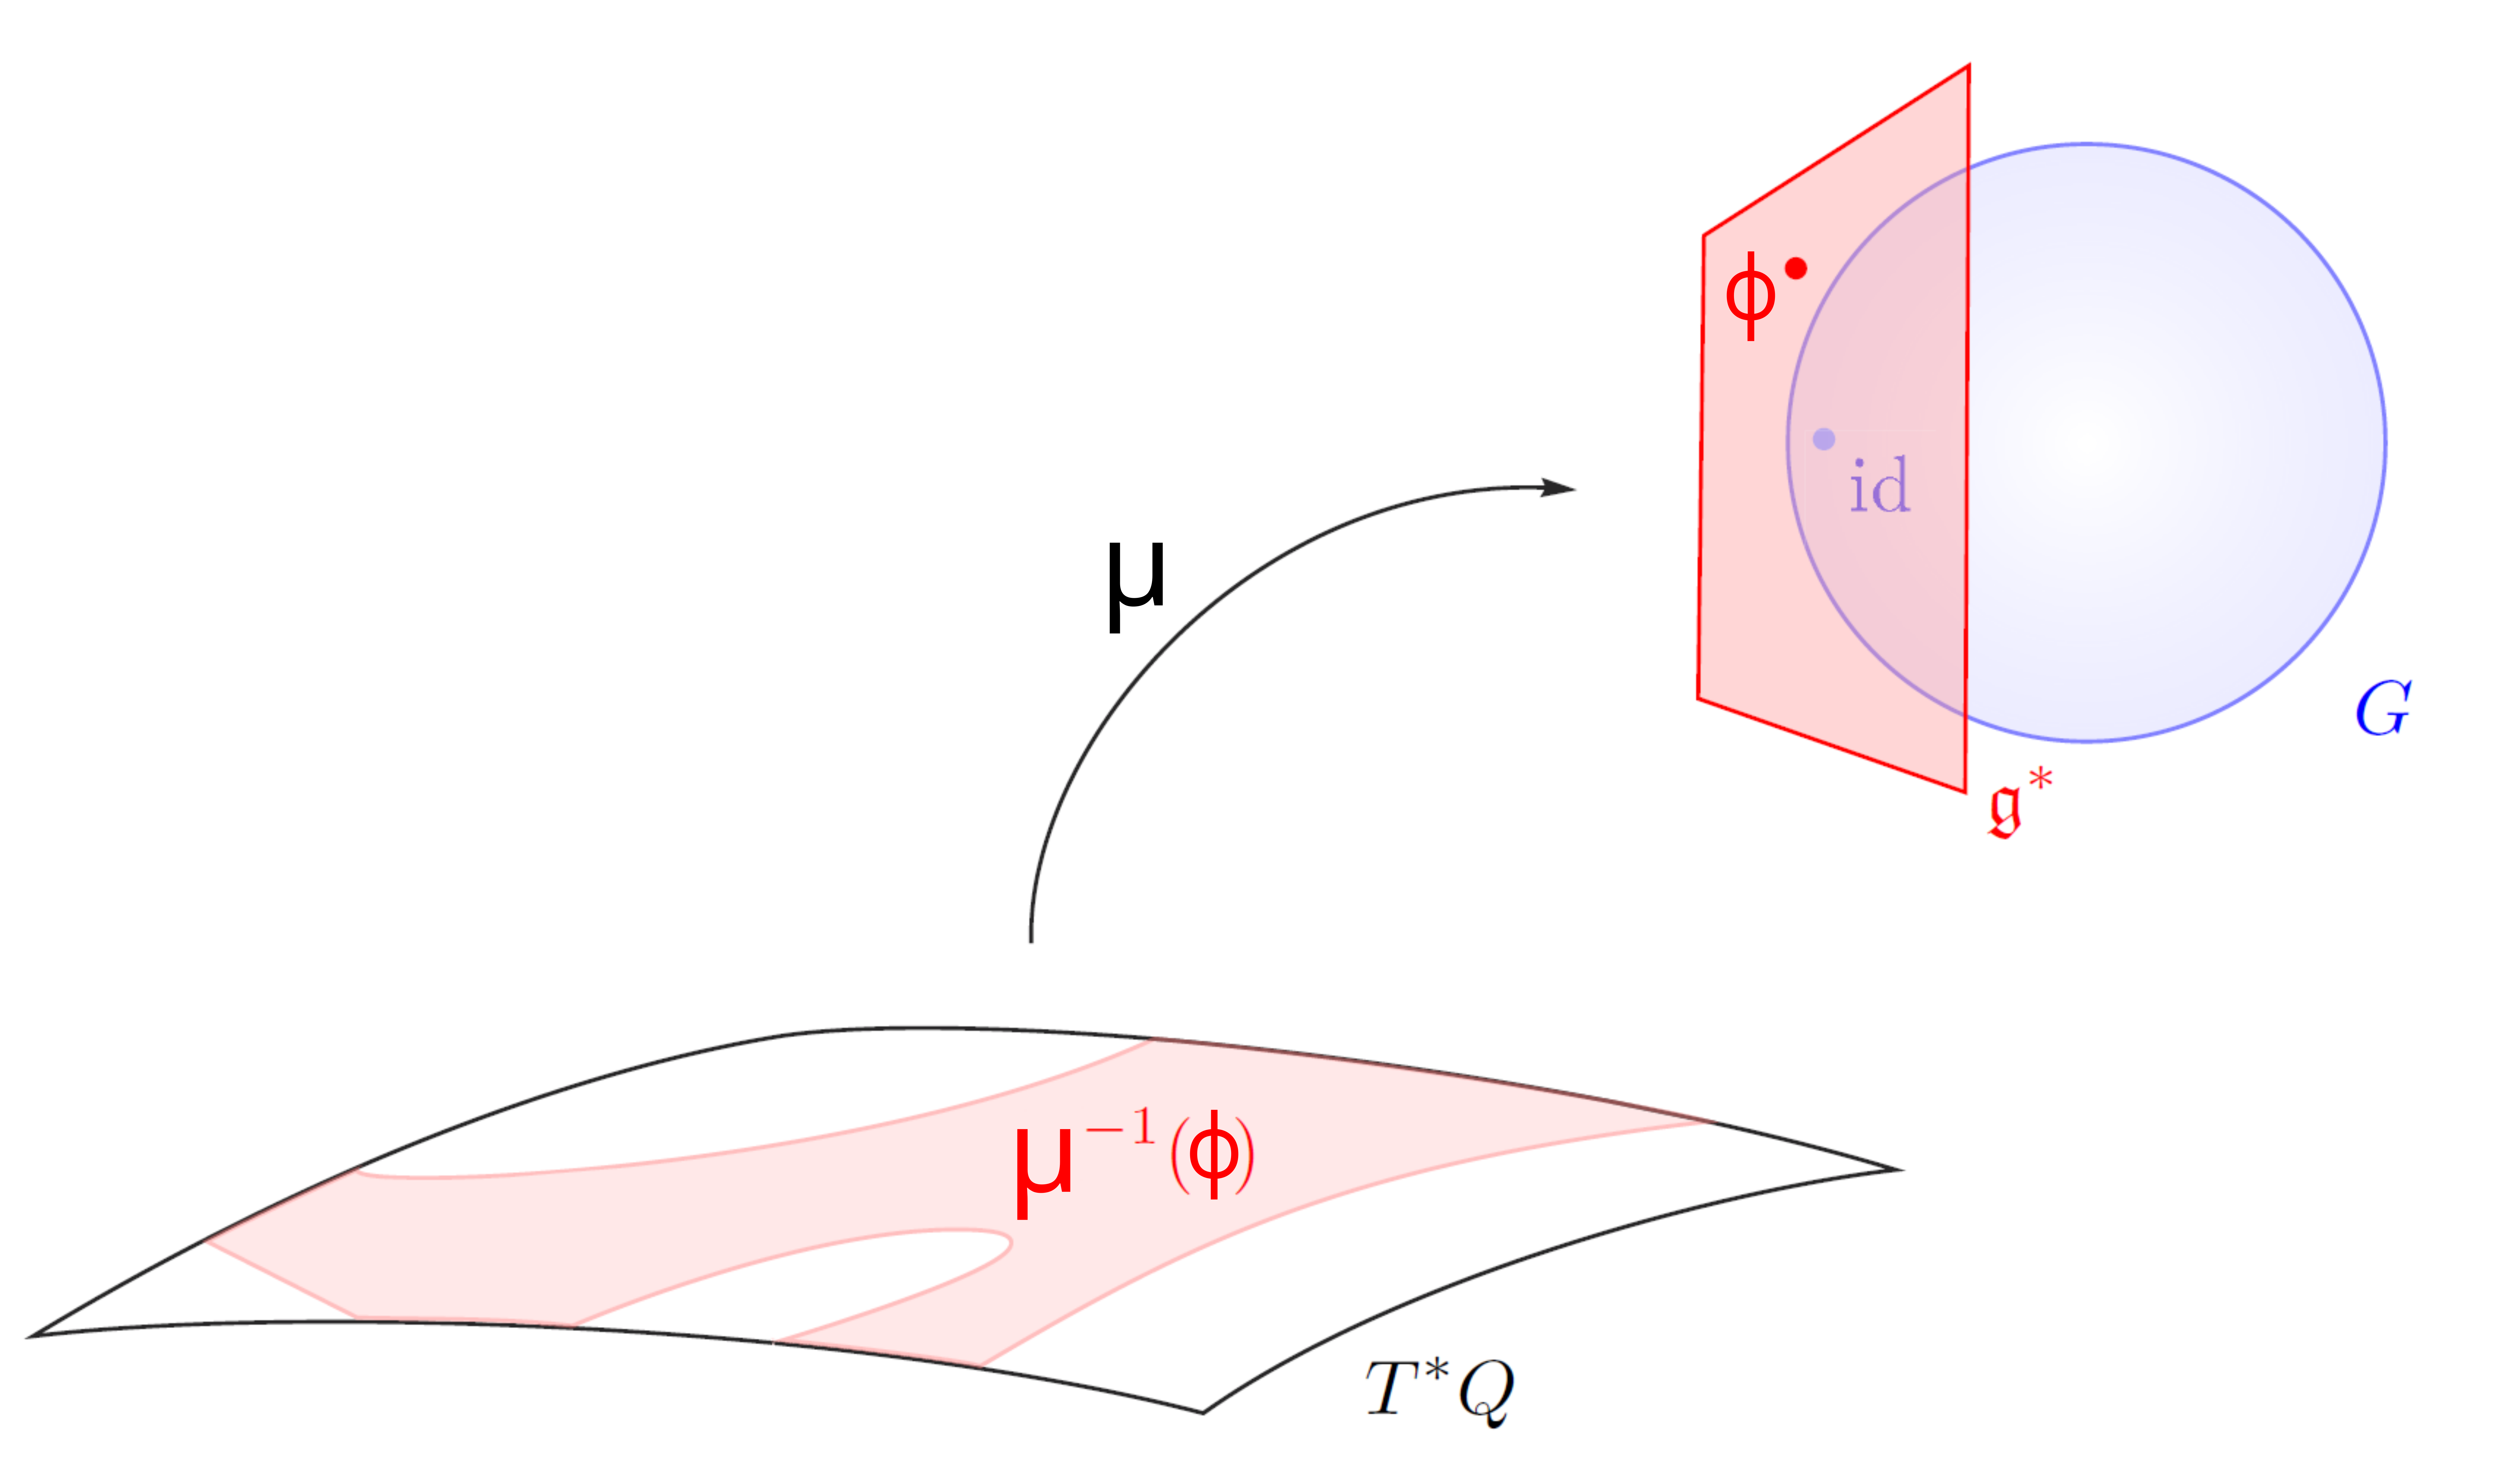
\includegraphics[width=\textwidth]{Pictures/Reduction}
		\end{column}	
		
		\begin{column}{0.6\textwidth}
				\textbf{\color{UniGreen}In mechanics:}~~
				\\
			{\it \small
				it embodies the process of restricting the dynamics of the system to the level sets of the conserved quantities pertaining to the symmetry group.		
			}
			\\[.2em]
			\color{gray}\small( e.g. restricting to studying a point-like particle in a central potential by studying it in radial coordinates)
		\end{column}	
	\end{columns}	
\end{frame}
\note[itemize]{
	\item
}
%------------------------------------------------------------------------------------------------

\subsection{Regular reduction in multisymplectic geometry}
%------------------------------------------------------------------------------------------------
\begin{frame}{Momentum maps in multisymplectic geometry}
	Consider $\theta:G\curvearrowright M$ {\color{UniGreen}multi}symplectic,~~ $\underline{\cdot}:\mathfrak{g}\to \mathfrak{X}(M)$ infinitesimal action.
	\vfill

	\begin{columns}[T]
		\setlength{\belowdisplayskip}{5pt}
		\begin{column}{.50\linewidth}
			%
			\centering \it
			\onslide<2->{
				\begin{defblock}[Equivariant moment map]
					Smooth map $$\mu:M\to \mathfrak{g}^\ast{\color{UniGreen}\otimes \Lambda^{n-1}T^\ast M}$$
					such that:
					\begin{itemize}
						\item[i.] $d\langle \mu,\xi\rangle = -\iota_{\underline{\xi}}\omega$ \qquad\qquad \small,$\forall \xi \in \mathfrak{g}$
						\item[ii.] $\mu \circ \theta_g = \left(Ad_g^\ast {\color{UniGreen} \,\otimes\, \theta^\ast_g}\right) \circ \mu$ \quad \small, $\forall g \in G$
						\item[iii.] {\color{UniGreen} $\mu \in \Omega^{n-1}(M,\mathfrak{g})$}
					\end{itemize}
				\end{defblock}
			}
		\end{column}	
		%
		\onslide<2->{\vrule{}}
		%
		\begin{column}{.50\linewidth}
			\onslide<3->{			
				\begin{defblock}[Comoment map]
					Linear map $$\widetilde{\mu}: \mathfrak{g}\to {\color{UniGreen}Leib(M,\omega)}$$
					such that:
					\begin{itemize}
						\item[i.] $d\widetilde{\mu}(\xi) = -\iota_{\underline{\xi}}\omega$ 
						\qquad~\small, $\forall \xi \in \mathfrak{g}$
						\item[ii.] $\widetilde{\mu}([\xi,\eta]) = \lbrace\widetilde{\mu}(\xi),\widetilde{\mu}(\eta)\rbrace$ \small, $\forall \xi,\eta \in \mathfrak{g}$
					\end{itemize}
				\end{defblock}
			}
		\end{column}	
	\end{columns}	
	%
	\pause
	\vspace{.5em}
	%
	\begin{columns}[]
		\setlength{\belowdisplayskip}{5pt}
		\begin{column}{.40\linewidth}
			%
			\centering \it
			\onslide<5->{
				\begin{upshotblocktitle}[Duality]
					\begin{displaymath}
						\mu(x) : \mathfrak{\xi} \mapsto \widetilde{\mu}(\xi)\big\vert_x
					\end{displaymath}
					%
					\emph{
					\small
					"duality wrt. the currying operation"					
					}
				\end{upshotblocktitle}
			}
		\end{column}	
		%
		%
		\begin{column}{.60\linewidth}
			\onslide<4->{			
				\begin{upshotblocktitle}[$\widetilde{\mu}$ as a lift]
					\begin{displaymath}
						\begin{tikzcd}[ampersand replacement = \&]
						 \& {\color{UniGreen}Leib(M,\omega)} \ar[d,"\vHam"]
						 \\
						 \mathfrak{g} \ar[ur,dashed,sloped,"\widetilde{\mu}"]\ar[r,"\underline{\cdot}"'] \& \mathfrak{X}(M)
						\end{tikzcd}
					\end{displaymath}
					%
					\emph{
					\small
					"it is a lift (in the {\color{UniGreen}Leibniz} category) of the infinitesimal action by the assigment of hamiltonian v.fields."					
					}
				\end{upshotblocktitle}
			}
		\end{column}	
	\end{columns}		
\end{frame}
\note[itemize]{
	\item consider an action preserving the symplectic form.
	\item details:
	\begin{itemize}
		\item[-] $\langle \cdot, \cdot \rangle$ is the natural pairing of $\mathfrak{g}$ and $\mathfrak{g}^\ast$.
		\item[-] $\theta_g$ is the diffeomorphism associated to $g\in G$ via $\theta:G\curvearrowright M$
		\item[-] $Ad^\ast_g$ is the coadjoint action $G\curvearrowright \mathfrak{g}^\ast$
		\item[-] $\theta^\ast_g$ is the induced action $G\curvearrowright \Lambda^{n-1}T^\ast M$ (lift on differential forms)

	\end{itemize}
	\item The moment map can be reexpressed as a comomentum map.
	\item Observe that ii. on the left always implies ii. on the right. The converse is trure only if $G$ is connected.
	\item $G\curvearrowright M$ is said "Hamiltonian" iff it admits comoment map $\widetilde{\mu}$.
}
%------------------------------------------------------------------------------------------------

%------------------------------------------------------------------------------------------------
\begin{frame}{Regular reduction in multisymplectic geometry}
	Let $(M,\omega)$ be $n$-plectic.
	Consider an action $G\curvearrowright M$ with moment map $\mu$.

	\pause
	\vfill
	\begin{defblock}[Regular value of $\mu$]
		Closed differential form $\phi \in \Omega^{n-1}(M,\mathfrak{g}^\ast)$, such that
		$$
		 \mu^{-1}(\phi)=\lbrace x \in M ~ \vert ~ \mu(x)=\phi(x)\rbrace
		$$
		is a smoothly embedded into $M$.	
	\end{defblock}	
	
	\pause
	\vfill
	

	\begin{thmblock}[Multisymplectic regular reduction \cite{Blacker20}]
		\vspace{-.4em}\hspace{-1em}
		\begin{tabular}{l p{14cm}}
		    Given: & $(M,\omega)$ {\color{UniGreen}$n$-}plectic
		    \\
		    & $G\curvearrowright M$ {\color{UniGreen}multi}symplectic with equivariant momap. {\color{UniGreen}$\mu\in \Omega^{n-1}(M,\mathfrak{g}^*)$}
		    \\[.2em]
		    Assume: & $\phi \in {\color{UniGreen} \Omega^{n-1}(M,\mathfrak{g}^*)}$ regular value of $\mu$ 
		    \quad\quad \footnotesize \textcolor{gray}{($\mu^{-1}(\phi)\hookrightarrow M$ embedding)}
		    \\
			& $G_\phi\curvearrowright \mu^{-1}(\phi)$ free and proper
			\quad\qquad \footnotesize \textcolor{gray}{($\mu^{-1}(\phi)/G_\phi$ smooth manifold)}
			\\[.4em]
			Then: & $\exists!$ {\color{UniGreen}pre-n-}plectic structure $\omega_\phi$ in $M_\phi:= \mu^{-1}(\phi)/G_\phi$ \\
			& s.t. $\pi^\ast \omega_\phi = j^\ast \omega$ 
			\qquad {\footnotesize with $j:\mu^{-1}(\phi) \hookrightarrow M$ and $\pi:\mu^{-1}(\phi)\twoheadrightarrow M_\mu$}
		\end{tabular}
		\vspace{-.4em}
	\end{thmblock}	
	
\end{frame}
\note[itemize]{
	\item First: introduce the higher analague of a "regular value" for the higher comomentum map.
	\item The notion of $G$-equivariant covariant moment map turns out to be the right prerequisite for reduction in the multisymplectic setting. Somewhat surprisingly, this is true, even for the ($L_\infty$-)algebraic reduction, where one might expect homotopy moment maps, which directly interact with the involved $L_\infty$-structures to play a role.
	\item pre-$n$-plectic means closed and possibly degenerate.
}
%------------------------------------------------------------------------------------------------


%------------------------------------------------------------------------------------------------
% Frame inspired by Leonid: passing from moment maps to comoment maps
\begin{frame}[fragile]{Reminder: Moment maps in symplectic geometry}
	Let $(M,\omega)$ be a symplectic manifold, $\vartheta: G\times M \to M$ a Lie group action preserving $\omega$ and $v:\mathfrak{g}\to \mathfrak{X}(M)$ the corresponding infinitesimal action
	%
		\begin{defblock}[Moment map pertaining to $\vartheta$]
			Smooth map $ \mu: M \to \mathfrak{g}^\ast$ such that: \stackunder{$d \langle\mu , \xi \rangle = \iota_{v_\xi}\omega \scriptstyle\quad \forall \xi \in \mathfrak{g}$}{$f (\vartheta_g(x)) = Ad^\ast_g (f(x)) \scriptstyle\quad \forall g \in G, x \in M$}
		\end{defblock}
	%
	\vfill
	\emph{... from a dual perspective (assuming $G$ connected) ...}
			\begin{defblock}[Comoment map pertaining to $v$]
				\begin{columns}
					\begin{column}{.5\linewidth}	
			Lie algebra morphism \qquad $ f: \mathfrak{g} \to C^\infty(M) $
			\\
			such that \qquad $ d~f (x) = -\iota_{v_x} \omega \qquad \forall x \in \mathfrak{g}~.$
					\end{column}
					\begin{column}{.4\linewidth}	
						\begin{displaymath}
							\begin{tikzcd}
								& C^{\infty}(M,\omega) \ar[d]
								\\
								\mathfrak{g} \ar[ur,dashed,"(f)"]\ar[r,"v"']& \mathfrak{X}(M)
							\end{tikzcd}	
						\end{displaymath}
					\end{column}
				\end{columns}
		\end{defblock}		
	%
	\vfill
	\emph{... a tool encoding conserved quantities ...}
	\begin{propblock}[Noether Theorem]
		\small Fixed $H\in C^\infty_{\text{Ham}}(M)$ ($\mathfrak{g}$-invariant) ,
				$$\mathcal{L}_{v_H} f(x) = 0 \qquad \forall x \in \mathfrak{g}$$
	\end{propblock}
\end{frame}
\note[itemize]{
	\item comoment map is a Lie algebra morphism projecting to $v$. (Triangle diagram in Lie algebra category).
}



%------------------------------------------------------------------------------------------------
\begin{frame}{Geometry of symmetries}\label{frame:geometrysymmetries}
	Basic mechanical structures are encoded in geometry. but there is another complementary geometrical property that's natural in physics: symmetry!
	\begin{alertblock}{Upshot}
		Continous symmetries are described by actions of a Lie group on $M$.
	\end{alertblock}
	\begin{block}{Noether}
		Presence of symmetries $\quad \Rightarrow \quad$ existence of conserved quantities.
	\end{block}	
	\begin{block}{Key concept:}
		Noether current are encoded in a \emph{moment map}  $\mu :M \rightarrow \mathfrak{g}^*$ (the dual of the comoment map $f$. 
	\end{block}
  \begin{columns}[T]
   	\begin{column}{.6\textwidth}
			\begin{block}{Symplectic reduction:}
			\begin{itemize}
				\item System dynamics should be restricted to level set of conserved observables in order to efficiently store dynamical properties.
				\item Under certain assumptions, $\mu^{-1}( 0 )/G$ is a symplectic manifold with an "induced" symplectic structure.
			\end{itemize}
			\end{block}
    \end{column}
    \begin{column}{.4\textwidth}	
			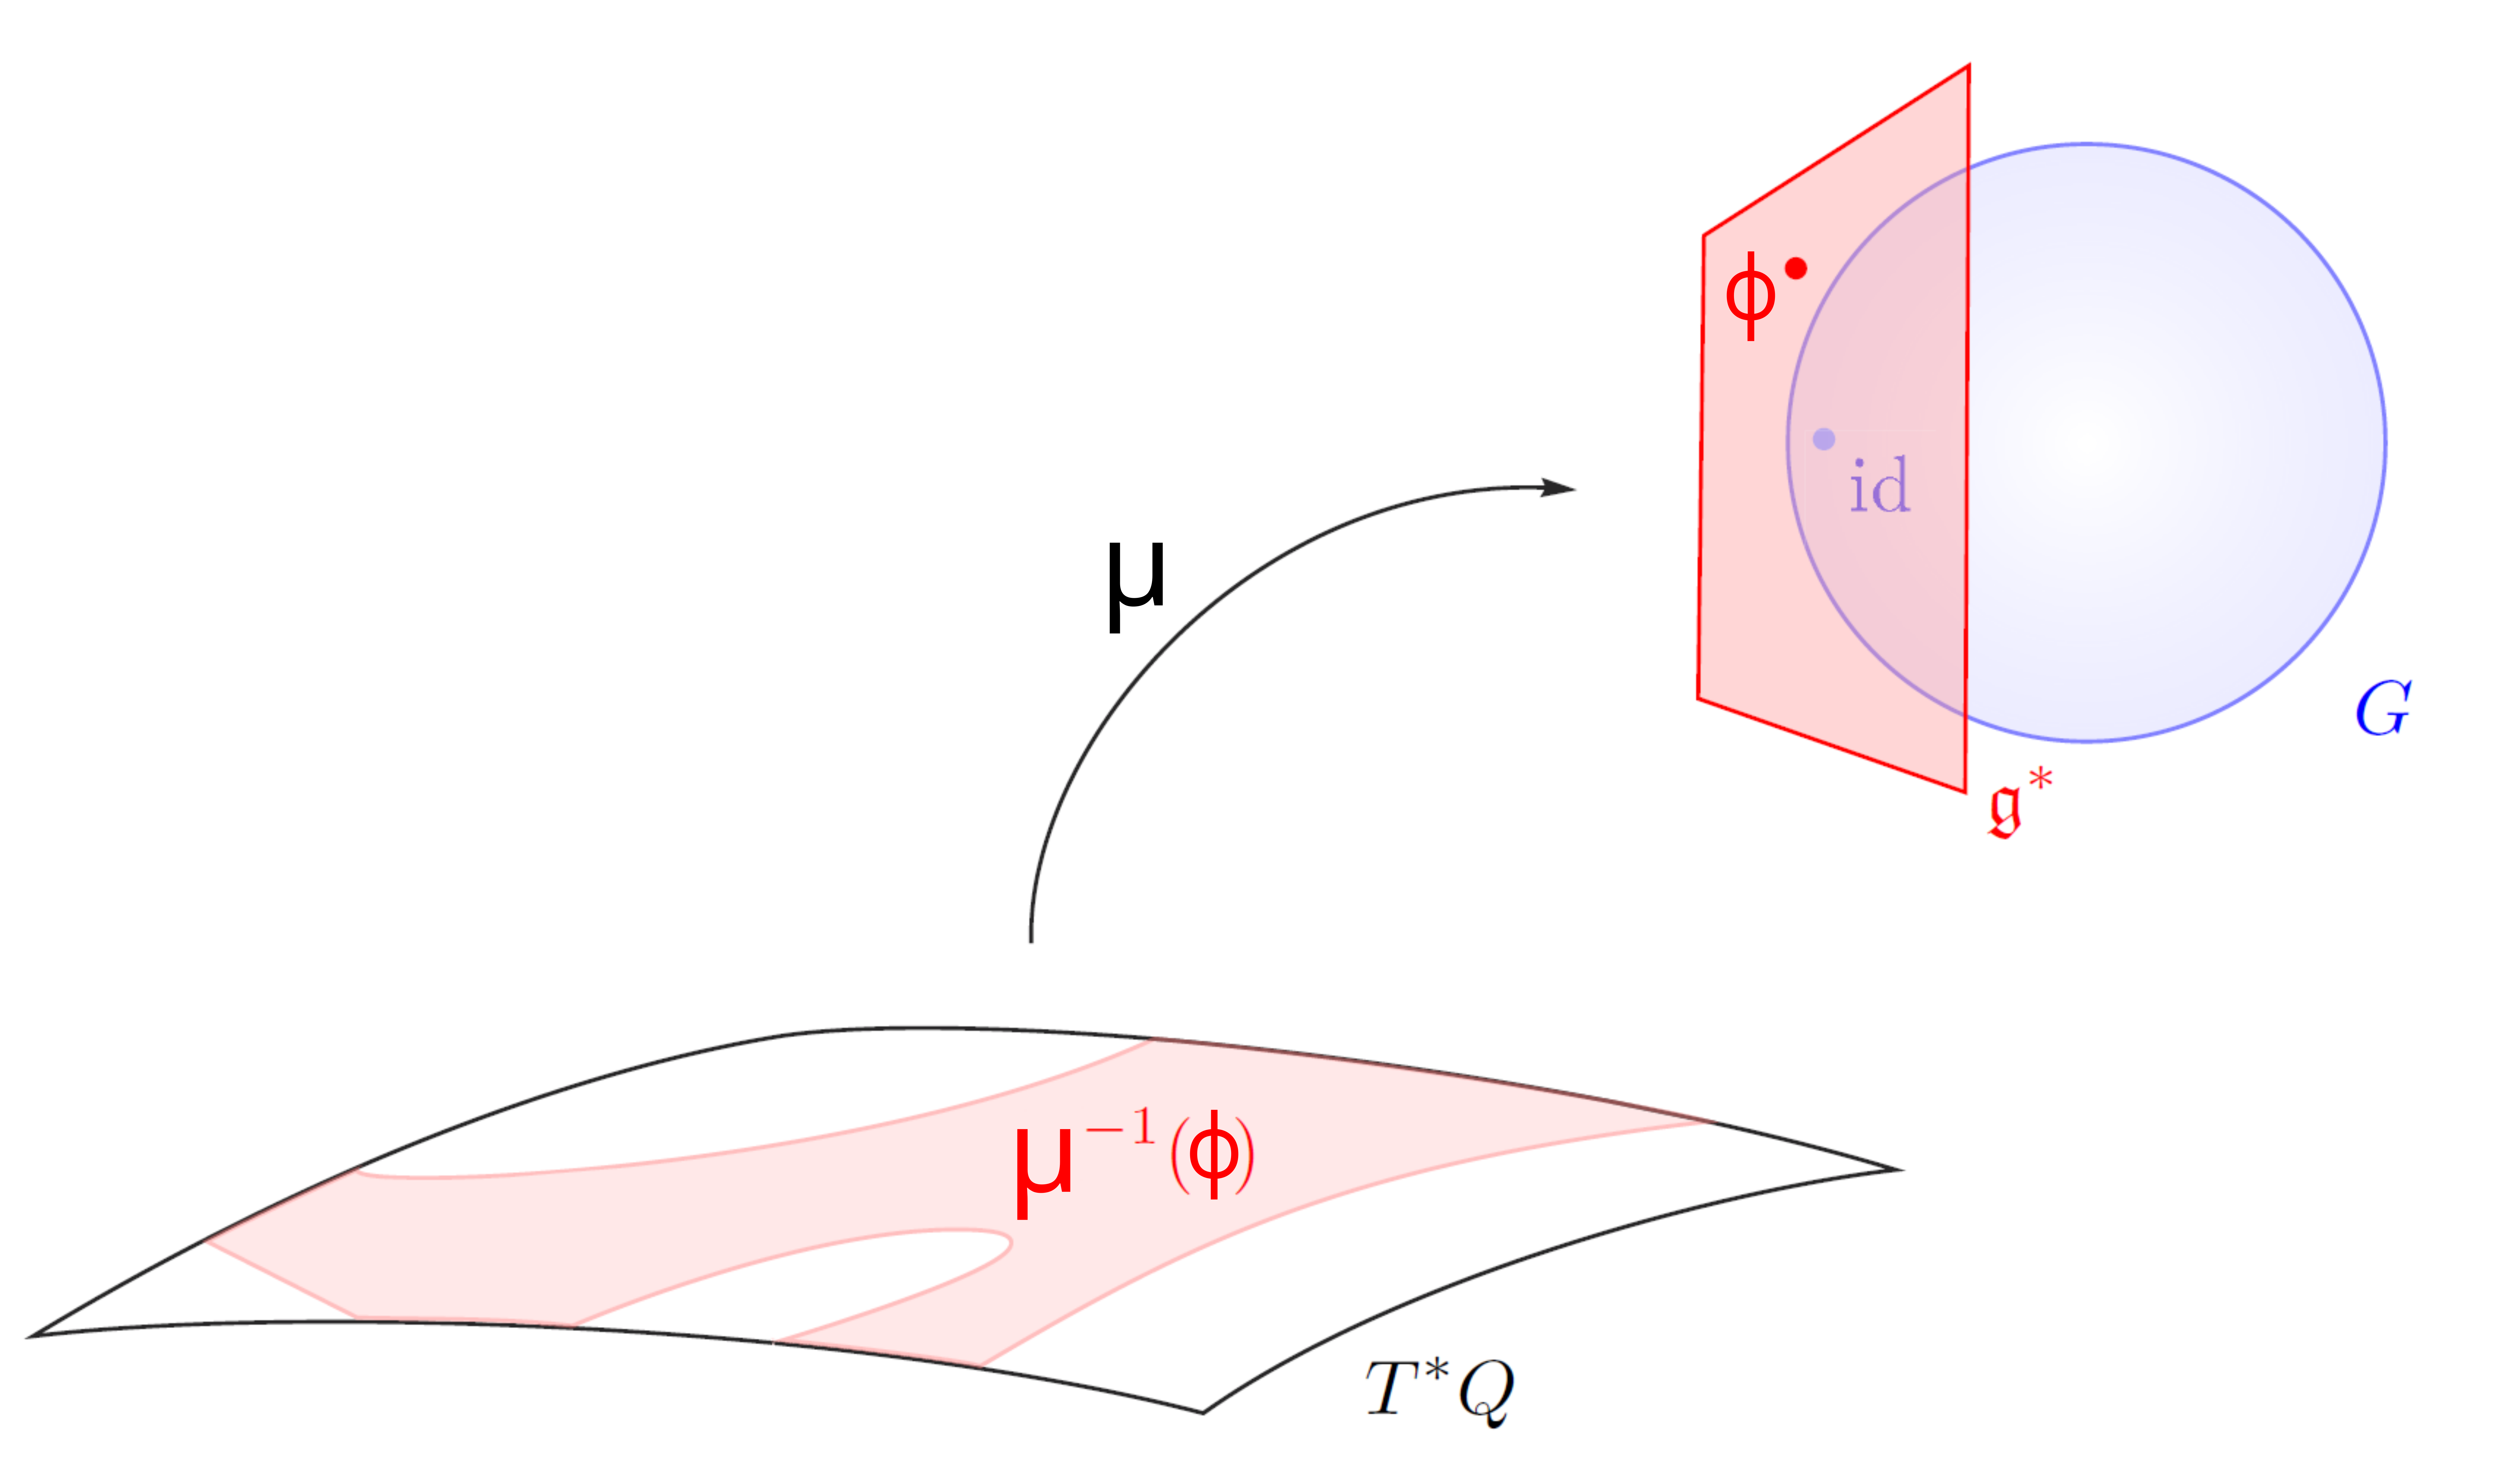
\includegraphics[width=\textwidth]{Pictures/Reduction} 
  	\end{column}
	\end{columns}			
\end{frame}
\note{
}
%------------------------------------------------------------------------------------------------



%---------------------------------------------------------------------------------------------------------------------------------------------------
\begin{frame}{Research proposal context: (multi)symplectic reduction}



\end{frame}
\note{
}
%---------------------------------------------------------------------------------------------------------------------------------------------------


%-------------------------------------------------------------------------------------------------------------------------------------------------
\begin{frame}[t]{Symmetries in \textbf{multisymplectic geometry}}
	Consider a Lie algebra action $v:\mathfrak{g} \to \mathfrak{X}(M)$  preserving the $n$-plectic form $\omega$,
	\vfill

	\vspace{-1em}
	\begin{columns}[T]
		\setlength{\belowdisplayskip}{5pt}
		\begin{column}{.50\linewidth}
			%
			\centering \it
			\onslide<2->{
				$-$ symplectic case $-$
				\begin{defblock}[Comoment map pertaining to $v$]
					Lie algebra morphism
					$$ f: \mathfrak{g} \to C^\infty(M) $$
					such that
					$$ d~f (x) = -\iota_{v_x} \omega \qquad \forall x \in \mathfrak{g}~.$$
				\end{defblock}
			}
		\end{column}	
		%
		\onslide<2->{\vrule{}}
		%
		\begin{column}{.50\linewidth}
			\centering \it
			\onslide<3->{			
				$-$ $n$-plectic case $-$
				\begin{defblock}[Homotopy comoment map \tiny (HCMM)]
					$L_\infty$-morphism 
					$$ (f_k) : \mathfrak{g} \to L_\infty (M,\omega)$$
					such that
					$$ d~f_1(x) = -\iota_{v_x} \omega \qquad \forall x \in \mathfrak{g}~.$$
				\end{defblock}	
			}
		\end{column}	
	\end{columns}	
	%
	\pause
	\vfill
	\centering 
	\onslide<4->{\textbf{-- Conserved quantities --}}
	%
	\vspace{-.5em}
	\begin{columns}[T]
		\setlength{\belowdisplayskip}{5pt}
		\begin{column}{.50\linewidth}
			%
			\centering \it
			\onslide<4->{
			\begin{propblock}[Noether Theorem]
				\small Fixed $H\in C^\infty_{\text{Ham}}(M)$ ($\mathfrak{g}$-invariant) ,
				$$\mathcal{L}_{v_H} f(x) = 0 \qquad \forall x \in \mathfrak{g}$$
			\end{propblock}
			}
		\end{column}	
		%
		\onslide<5->{\vrule{}}
		%
		\begin{column}{.50\linewidth}
			\centering \it
			\onslide<5->{			
			\begin{propblock}[RWZ16 Theorem]
				\small Fixed $H\in \Omega^{n-1}_{\text{Ham}}(M)$ ($\mathfrak{g}$-invariant),
				$$\mathcal{L}_{v_H} f_k(p) \in B^k(M) \qquad \forall p \in Z_k(\mathfrak{g})$$			
			\end{propblock}
			}
		\end{column}	
	\end{columns}		
\end{frame}
\note{
}
%-------------------------------------------------------------------------------------------------------------------------------------------------


\end{document}